\section{Graph Parsing Algorithm}

We propose graph parsing algorithm which allows to create finite representation of parse forest which contains trees for all satisfied paths in graph.
Finite representation of result set with structure related to specified grammar may be useful not only for results understanding and processing but also for query debugging especially for complex queries. 

Therefore our solution is based on generalized LL (GLL)~\cite{scott2010gll, FastPracticalGLL} parsing algorithm which allows to process arbitrary (including left-recursive and ambiguous) context-free grammars with worst-case cubic time complexity and linear for LL grammars. 

\subsection{Generalized LL Parsing Algorithm}

In classical LL algorithm we have a pointer to input (position $i$) and a pointer to grammar in form $n \rightarrow \alpha \cdot x \beta $ --- grammar slot.
The parsing may be described as a movement of this pointers from initial position: $i=0$, $s \rightarrow \cdot \beta $, where $s$ is start nonterminal. Thus in each step we have two pointers and some possible cases to process them. 

\begin{enumerate}
\item $n \rightarrow \alpha \cdot x \beta $ when $x$ is a terminal and $x = input[i]$. In this case we should move both pointers right: $i = i + 1$, new slot $= n \rightarrow \alpha  x \cdot \beta $.
\item $n \rightarrow \alpha \cdot x \beta $ when $x$ is nonterminal. In this case we should save return address $n \rightarrow \alpha x \cdot \beta $ in stack and move pointer in grammar to position $x \rightarrow \cdot \gamma$.\label{itm:2}
\item $n \rightarrow \alpha \cdot $. This case means that we finish processing of nonterminal $n$. We should pop return address from stack and use it as new slot.\label{itm:3}
\item $s \rightarrow \alpha \cdot $ where $s$ is a start nonterminal of grammar. In this case we should check emptiness of input and report success or failure. 
\end{enumerate}

In case~\ref{itm:2} we can use $FIRST$ set to choose single variant. 
But sometimes it is not possible to select only one path to continue parsing and it does not allow to use LL parsing algorithm.
Generalized LL algorithm handles all possible paths in this case. 
Instead of immediate processing of all variants, GLL uses descriptors mechanism to store all possible branches and process them sequentially. 
Descriptor is a quadriple $(L, s, j, a)$ where $L$ is a grammar slot, $s$ is a stack node, $j$ is a position in the input, and $a$ is a node of derivation tree. 

The stack in parsing process is used to store return information for the parser --- a name of function which would be called when current function will finish computation. 
As mentioned before, generalized parsers process all possible derivation branches and for every branch parser must store it's own stack. It leads to infinite stack growth.  
Tomita-style graph structured stack (GSS)~\cite{Tomita} allows to combine stacks to solve this problem.
In GLL each GSS node contains a pair of position in input and grammar slot. 

In order to provide termination and correctness we should avoid duplication of descriptors, and allow to process GSS nodes in arbitrary order. It is necessary to use some additional sets for this.
\begin{itemize}
\item $R$ --- working set which contains descriptors to process. Algorithm finish when $R$ is empty.
\item $U$ --- all descriptors was created. Avoid duplication of these.
\item $P$ --- popped nodes. Allows to process descriptors (and GSS nodes) in arbitrary order without loosing new descriptors in step~\ref{itm:3}. 
\end{itemize}

Instead of explicit code generation used in classical algorithm, we use table version of GLL~\cite{TableGLL} in order to simplify adaptation to graph processing.
As a result, main control function is different from the original one because it should process LL-like table instead of switching between generated parsing functions.
Control functions of the table based GLL are presented in listing~\ref{mainTblFunctions}. All other functions are the same as in original algorithm and their description can be found in original article~\cite{scott2010gll} or in Appendix~\ref{GLLCode}.

\begin{algorithm}[h]
\begin{algorithmic}[1]
\caption{Control functions of table version of GLL}
\label{mainTblFunctions}
\Function{dispatcher}{}
  \If{$R.Count \neq 0$}  
      \State{$(L,v,i,cN) \gets R.Get()$}
      \State{$cR \gets dummy$}
      \State{$dispatch \gets false$}
  \Else
      \State{$stop \gets true$}
  \EndIf
\EndFunction

\Function{processing}{}
  \State{$dispatch \gets true$}
  \Switch{$L$}
  \Case{$(X \rightarrow \alpha \cdot x \beta)$ where $x = input[i + 1])$}
       \If{$cN = dummyAST$} 
          \State{$cN \gets \Call{getNodeT}{i}$} 
       \Else 
          \State{$cR \gets \Call{getNodeT}{i}$}
       \EndIf
       \State{$i \gets i + 1$}
       \State{$L \gets (X \rightarrow \alpha x \cdot \beta)$}
       \If{$cR \neq dummy$}
          \State{$cN \gets \Call{getNodeP}{L, cN, cR}$} 
       \EndIf
       \State{$dispatch \gets false$}        
  \EndCase
  \Case{$(X \rightarrow \alpha \cdot x \beta)$ where $x$ is nonterminal}
       \State{$v \gets$ \Call{create}{$(X \rightarrow \alpha x \cdot \beta), v, i, cN$}}
       \State{$slots \gets pTable[x][input[i]]$}
       \ForAll{$L \in slots$}
          \State{\Call{add}{L,v,i,dummy}} 
       \EndFor
  \EndCase
  \Case{$(X \rightarrow \alpha \cdot )$}
       \State{\Call{pop}{v,i,cN}} 
  \EndCase
  \Case{$(S \rightarrow \alpha \cdot )$ when $S$ is start nonterminal}
       \State{final result processing and error notification} 
  \EndCase
  \EndSwitch
\EndFunction

\Function{control}{}
  \While{not $stop$}  
      \If{$dispatch$}
        \State{\Call{dispatcher}{}}
      \Else
         \State{\Call{processing}{}}
      \EndIf
  \EndWhile
\EndFunction

\end{algorithmic}
\end{algorithm}

There are more than one tree for ambiguous grammar and generalized algorithms builds all derivation trees. Special data structure --- Shared Packed Parse Forest~\cite{SPPF} --- is used to reduce space required for tree storage.


\subsection{Shared Packed Parse Forest}

Binarized Shared Packed Parse Forest (SPPF)~\cite{brnglr} allows to compress derivation trees with optimal reusing of common nodes and subtrees.
Version of GLL which uses this structure for parsing forest representation achieves worst-case cubic space complexity~\cite{gllParsingTree}.

Let we present an example of SPPF for the input sentence \verb|"ABABAB"| and ambiguous grammar $G_0$ (pic~\ref{grammarG0}).

\begin{figure}[h]
   \begin{center}
\begin{verbatim}
   0: s = eps
   1: s = A s B
   2: s = s s
\end{verbatim}
   \caption{Grammar $G_0$}
   \label{grammarG0}        
   \end{center}
\end{figure}


There are two different leftmost derivations of given sentence in grammar $G_0$, hence SPPF should contains two different trees. Result SPPF(fig. ~\ref{sppf}) and two trees (fig.~\ref{tree1} and fig.~\ref{tree2}) are presented in figure~\ref{sppfSample}. 
 
\begin{figure*}[ht]
    \begin{center}
    \centering
    \begin{subfigure}[b]{0.3\textwidth}
        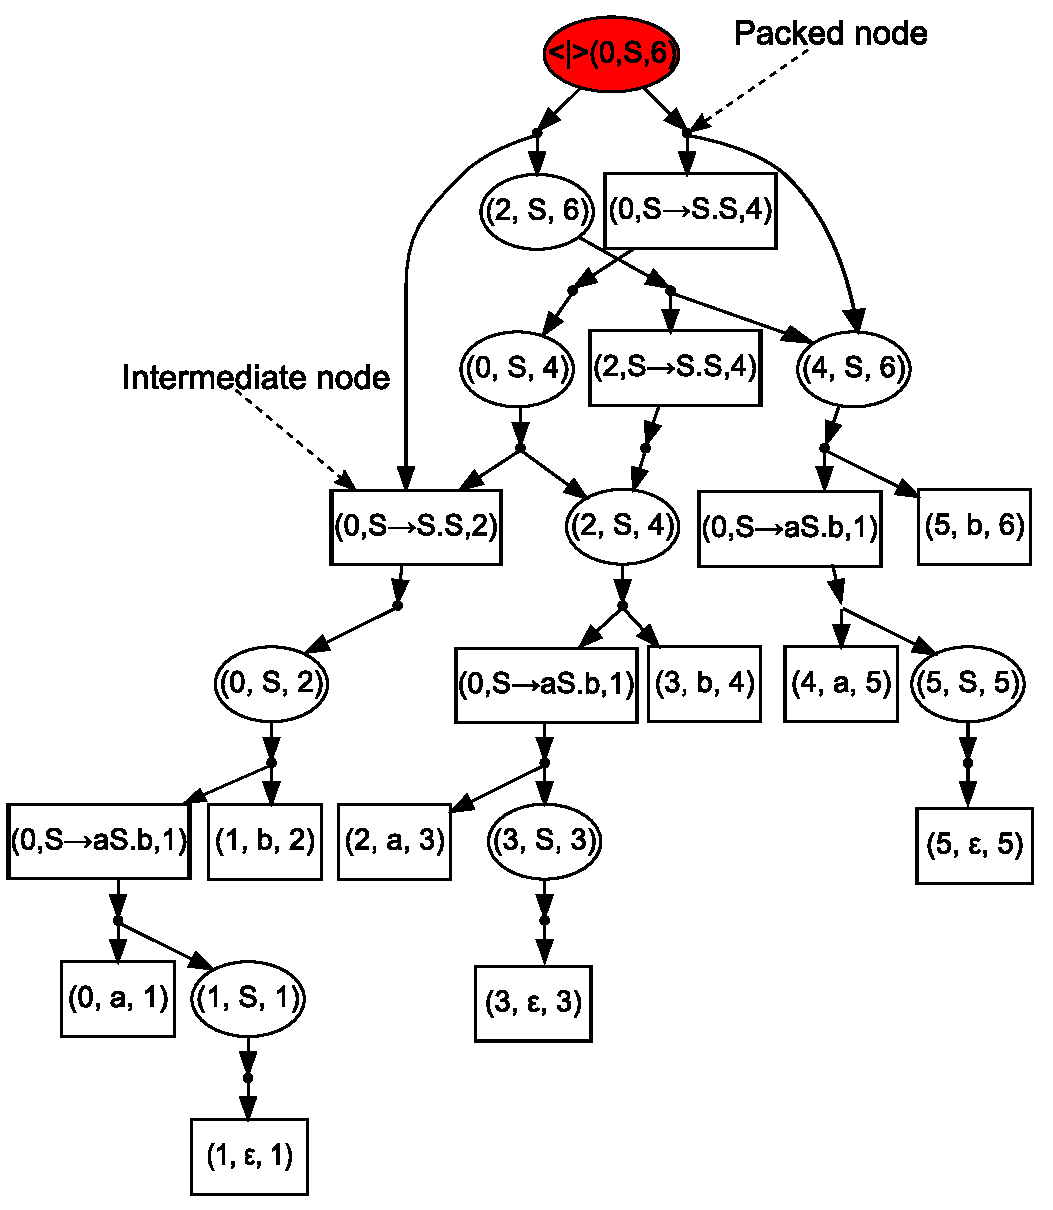
\includegraphics[width=\textwidth]{dot/Brackets.pdf}
        \caption{SPPF}
        \label{sppf}        
    \end{subfigure}
    ~
    \begin{subfigure}[b]{0.3\textwidth}
        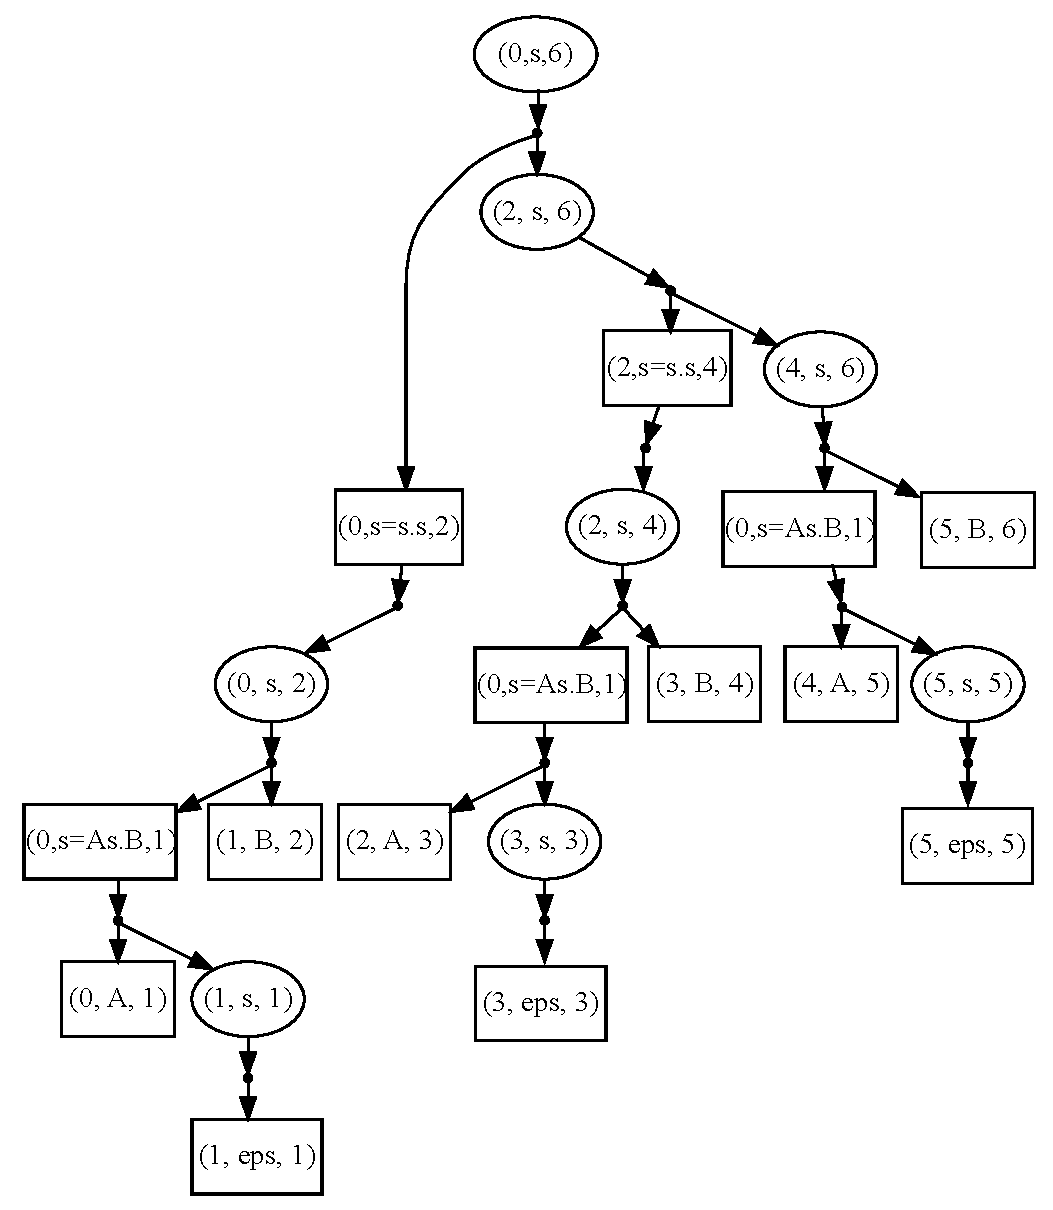
\includegraphics[width=\textwidth]{dot/Brackets1.pdf}
        \caption{First derivation tree}
        \label{tree1}        
    \end{subfigure}
    ~
    \begin{subfigure}[b]{0.3\textwidth}
        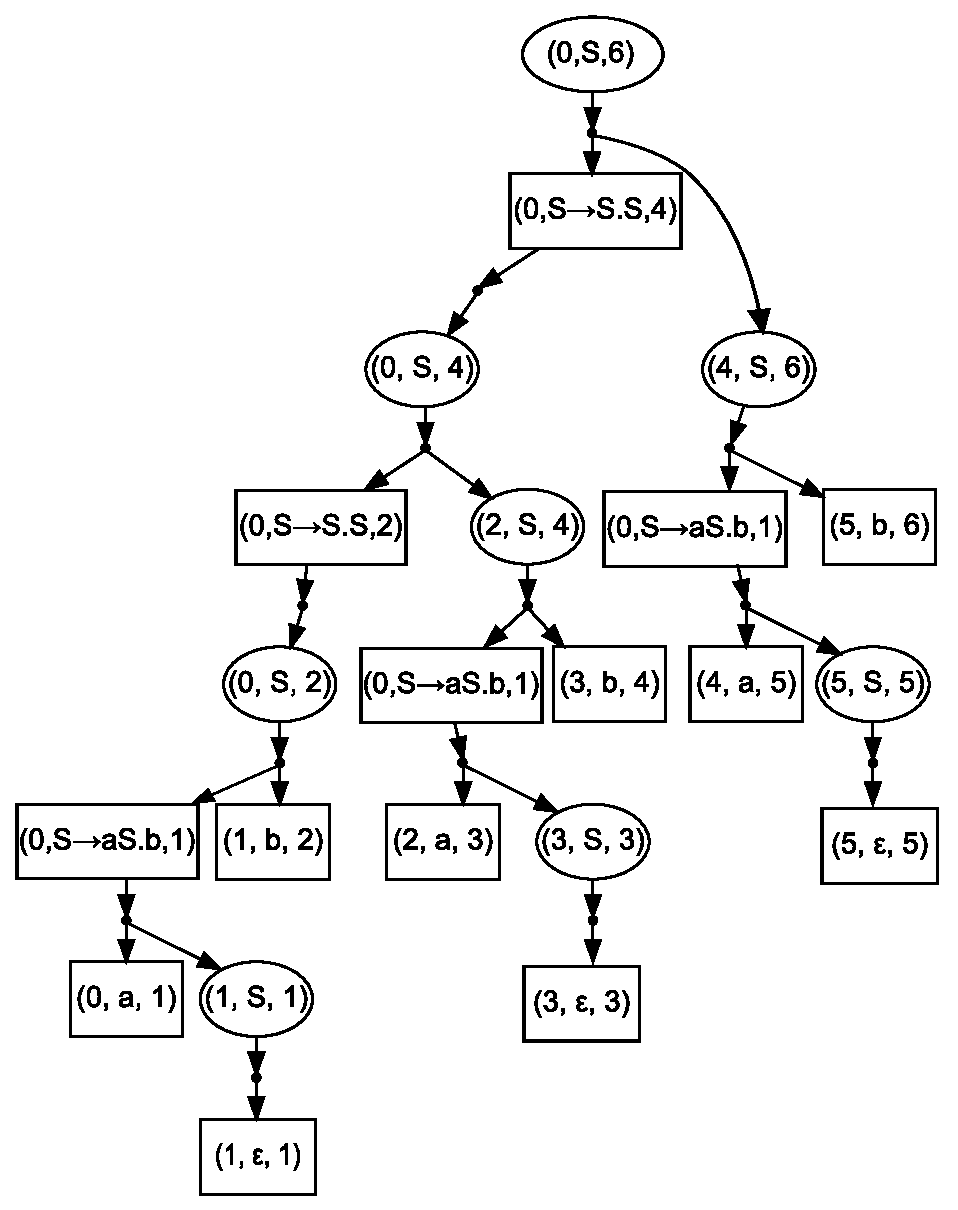
\includegraphics[width=\textwidth]{dot/Brackets2.pdf}
        \caption{Second derivation tree}
        \label{tree2}        
    \end{subfigure}
    \caption{SPPF for sentence \textbf{\texttt{"ABABAB"}} and grammar $G_0$}
    \label{sppfSample}
    \end{center}                
\end{figure*}

Binarised SPPF can be represented as a graph where each node has one of four types which described below with correspondent graphical notation.
Let $i$ and $j$ are start and end positions of substring, and tuple of positions $(i,j)$ is an \textit{extension} of node.

\begin{itemize}
    \item Node with rectangle shape labeled with $(i, T, j)$ is terminal node.     
    \item Node with oval shape labeled with $(i, N, j)$ is nonterminal node. 
    This node denotes that there is at least one derivation for substring $\alpha$ from position $i$ to position $j$ in input string $\omega$ such that $N \Rightarrow^*_G \alpha, \alpha = \omega[i..j-1] $.
    All derivation trees for given substring and nonterminal can be extracted from SPPF by left-to-right top-down graph traversal started from respective node. 
    We use filled nonterminal node labeled with $(<\mkern-11mu | \mkern-11mu> (i, N, j))$ for denote that there are more then one derivations from nonterminal $N$ for substring from $i$ to $j$.
    \item Packed node with label $(i,t,j)$ where $t$ is a grammar slot. We use dot shape for these nodes and omit label because it is important only for SPPF constriction.
    Subgraph with root in such node is one variant of derivation in case when parent is nonterminal node with label $(<\mkern-9mu | \mkern-9mu> (i, N, j))$.
    \item Node with rectangle shape and label $(N : \gamma \cdot, k)$ is an intermediate node.
\end{itemize}

Later in our examples we will remove redundant intermediate and packed nodes from the SPPF to simplify it and to decrease the size of structure.

\subsection{GLL-based Graph Parsing}

In this section we present such modification of GLL algorithm, that for input graph $M$, set of start vertices $V_s\subseteq V$, set of final vertices $V_f\subseteq V$, and grammar $G_1$
, it returns SPPF which contains all derivation trees for all paths $p$ in $M$, such that $\Omega(p) \in L(G_1)$, and $p.start \in V_s,\ p.end \in V_f$.
In other words, we propose GLL-based algorithm which can solve language constrained path problem.

First of all, notice that input string for classical parser can be represented as a linear graph, and positions in input are vertices of this graph.
This observation can be generalized to arbitrary graph with remark that for a position there is a set of labels of all outgoing edges for given vertex instead of just one next symbol. 
Thus, in order to use GLL for graph parsing we need to use graph vertices as positions in input and modify \textbf{Processing} function to allow to process multiple ``next symbols''.
Required modifications are presented in listing~\ref{modifAlgo}(line 5 and 17).
Small modification is also required for initialization of $R$ set: it is necessary to add not only one initial descriptor but the set of descriptors for all vertices in $V_s$.
All other functions can be reused from original algorithm without any changes.

\begin{algorithm}[h]
\begin{algorithmic}[1]
\caption{\textbf{Processing} function modified in order to process arbitrary directed graph}
\label{modifAlgo}
\Function{processing}{\ }
  \State{$dispatch \gets true$}
  \Switch{$L$}
  \Case{$(X \rightarrow \alpha \cdot x \beta)$ where $x$ is terminal}
       \ForAll{$\{ e | e \in input.outEdges(i), tag(e) = x \}$}
       \State{$new\_cN \gets cN$}
       \If{$new\_cN = dummyAST$} 
          \State{$new\_cN \gets \Call{getNodeT}{e}$} 
       \Else 
          \State{$new\_cR \gets \Call{getNodeT}{e}$}
       \EndIf
       \State{$L \gets (X \rightarrow \alpha x \cdot \beta)$}
       \If{$new\_cR \neq dummy$}
          \State{$new\_cN \gets \Call{getNodeP}{L, new\_cN, new\_cR}$} 
       \EndIf
       \State{\Call{add}{L,v,target(e),new\_cN}}
       \EndFor
  \EndCase
  \Case{$(X \rightarrow \alpha \cdot x \beta)$ where $x$ is nonterminal}
       \State{$v \gets$ \Call{create}{$(X \rightarrow \alpha x \cdot \beta), v, i, cN$}}
       \State{$slots \gets \bigcup_{e \in input.OutEdges(i)} pTable[x][e.Token]$}
       \ForAll{$L \in slots$}
          \State{\Call{add}{L,v,i,dummy}} 
       \EndFor
  \EndCase
  \Case{$(X \rightarrow \alpha \cdot )$}
       \State{\Call{pop}{v,i,cN}} 
  \EndCase
  \Case{$\_$}
       \State{final result processing and error notification} 
  \EndCase
  \EndSwitch
\EndFunction

\end{algorithmic}
\end{algorithm}

Note that our solution handles arbitrary numbers of start and final vertices, which allows to solve different kinds of problems arraising in the field
, namely all paths in graph, all paths from specified vertex, all paths between specified vertices. 
Also SPPF represents a structure of paths in terms of derivation which allows to get more useful information about result. 

Note that termination of proposed algorithm is inherited from the basic GLL algorithm.
We are process finite graphs, hence the set of positions is finite, and tree construction is not changed. 
As a result, total number of descriptors is finite, and any of them cannot be added in $R$ twice, hence main loop is finite.